\documentclass[12pt]{report}
\usepackage{amsmath}
\usepackage{amsfonts}
\usepackage{hyperref}
\usepackage{graphicx}
\usepackage{caption}
\usepackage{subcaption}
\setlength{\oddsidemargin}{0.5in}
\setlength{\evensidemargin}{0.5in}
\setlength{\textwidth}{6.0in}
\setlength{\topmargin}{.75in}
\setlength{\textheight}{8.6in}

\newcommand{\e}{\vec e}
\newcommand{\citeneeded}{}

% Modified by S. Aubin for the class of 2019 Physics theses

%
% This is a LaTeX template for an undergraduate honors or
%   senior thesis in physics at William & Mary. Created from
%   several theses from previous students of D.S. Armstrong,
%   pared down to bare bones.
%
%   you will need this present file (thesis_template.tex)
%   as well as the file  figure1.eps  to make the whole thing
%   (the latter is just an encapsulated postscript figure)
%     For simplicity, we don't use bibtex here; experts can choose
%   to use that more powerful way of dealing with citations.
%
%   To compile it, do:
% > pdflatex thesis_template.tex
% > pdflatex thesis_template.tex  (yes, you need to do it twice to
%                                  fill in the list of tables, figures
%                                  and references).

\begin{document}
\setlength{\baselineskip}{24pt}
\begin{titlepage}
\LARGE
\begin{center}
{\bf A Wonderful Piece of Scientific Research}\\[2.3cm]

\normalsize
A thesis submitted in partial fulfillment of the requirement \\
for the degree of Bachelor of Science with Honors in \\
Physics from the College of William and Mary in Virginia,\\[0.5cm]
by\\[0.5cm]
Stuart Thomas \\[2.5cm]
\end{center}
\normalsize
\begin{flushright}
%\hfill Accepted for Honors \\[.5cm]
\hfill \hrulefill \\
\hfill \hfill Advisor: Prof. Christopher J. Monahan\\[.6cm]
\hfill \hrulefill \\Prof. Todd Averett \\[.6cm]
\hfill \hrulefill \\Prof. Andreas Stathopoulos \\[.6cm]
\end{flushright}
\begin{center}
Williamsburg, Virginia\\
May 2021
\end{center}
\end{titlepage}

\setlength{\topmargin}{0.0in}

\pagenumbering{roman}
\tableofcontents
\chapter*{Acknowledgments}
\addcontentsline{toc}{chapter}{Acknowledgments}
\paragraph
\indent I would like to thank lots of people, and this is where
I will do it...


\listoffigures
\addcontentsline{toc}{chapter}{List of Figures}
\listoftables
\addcontentsline{toc}{chapter}{List of Tables}

\begin{abstract}
\setcounter{page}{5}
\addcontentsline{toc}{chapter}{Abstract}
\paragraph
\indent \textit{Abstract}

\end{abstract}

\pagenumbering{arabic}
\chapter{Introduction}

Quantum field theory (QFT) is an extraordinarily successful framework which can be applied to a range of physical phenomena. Paired with the Standard Model, QFT provides the prevailing basis for all small-scale physics (that is, where general relativity does not apply) and is the fundamental tool for studying particle physics. In condensed matter physics, effective field theories model emergent effects such as phonons and quasiparticles. Compared to experiment, QFT is remarkably accurate, famously matching the experimental value for the electron $g$-factor to eight significant figures.\cite{weisskopf1981} 

However, this power comes at a cost: the study of quantum fields is rife with infinities. A na\"ive treatment of quantum field theory produces divergent values for physical quantities, a clearly impossible result. Since the 1950s, this issue has been resolved for a large number of models--- most notably quantum electrodynamics--- through perturbation theory and the so-called \textit{renormalization group}. However, the technique fails with perturbatively nonrenormalizable theories. 

One such example is the \textit{non-linear sigma model}, a prototypical theory in both condensed matter and particle physics. In solid-state systems, this model describes Heisenberg ferromagnets and in nuclear physics, it acts as a prototype for quantum chromodynamics (QCD), exhibiting characteristic features such as a mass gap and asymptotic freedom. \citeneeded

In this study, we specifically consider the $O(3)$ non-linear sigma model in $1+1$ dimensions (one dimension of space, one dimension of time). This theory exhibits topological properties such as \textit{instantons}, or classical field solutions at local minima of the action.



Since the non-linear sigma model cannot be renormalized perturbatively, we cannot study these topological effects with normal perturbative techniques. An alternative solution is placing the field on a discretized lattice, a technique originally used for quantum chromodynamics. In this scenario, field configurations become computationally calculable. This process introduces an nonphysical length scale $a$, the lattice spacing. Therefore, we expect any physical result to converge in the continuum limit, i.e. when $a\rightarrow 0$. However, this is not always the case as observables mix on the lattice, leading to divergences. As an example, states of definite angular momentum mix when discretized, a clear violation of the angular momentum commutation relations. 


The gradient flow is a technique designed to remove these divergences. By dampening high-momentum fluctuations, the gradient flow reduces power-divergent mixing and make observables finite on the lattice.\cite{monahan2016} In quantum chromodynamics, previous studies have verified the ability of the gradient flow to make observables finite\citeneeded. Due to its success in QCD, there has been interest in using the gradient flow to finitize the topological susceptibility in the 1+1 $O(3)$ non-linear sigma model.\cite{bietenholz2018}.

%goals here

\section{Method Overview}

To numerically study the topological qualities of the non-linear sigma model, we first implement a Markov Chain Monte Carlo simulation. We initially construct a proof-of-concept Python program that models the simpler $\phi^4$ model (see Sec.~\ref{sec:phi4}). After comparing with existing literature, we transition to a C++ simulation for efficiency, implementing the non-linear sigma model in larger lattices. Since the gradient flow has no exact solution in the non-linear sigma model, we implement a numerical solution using a fourth-order Runge-Kutta approximation. By applying the gradient flow to every configuration in the sample, we can measure its effect on the topological charge and susceptibility.


\section{Conventions}
\begin{itemize}
    \item Throughout this paper, we use natural units, i.e. $\hbar = 1$ and $c=1$.
    \item We use Einstein summation notation, an implicit sum over repeated spacetime indices. For example, if $x^\mu$ is a spacetime four-vector and $x_\mu$ is its covariant form, the term
        \begin{align*}
            x^\mu x_\mu &= \sum^4_{\mu=0} x^\mu x_\mu \\
            &= x_0^2-x_1^2-x_2^2-x_3^2.
        \end{align*}
\end{itemize}

%\section{Main Experimental Goal}

\chapter{Theory}

This thesis incorporates two main bodies of knowledge: quantum field theory and statistical simulation. Through the path integral formulation of quantum field theory, we are able to describe the physics of the former with the established mathematics of the latter.

\section{Quantum Field Theory}


In this section we outline a rough description of quantum field theory. A full introduction is beyond the scope of this paper, however we do assume knowledge of nonrelativistic quantum mechanics and classical field theory.

The fundamental hypothesis of quantum field theory (QFT) describes particles as discrete packets of energy on a quantum field. But what is a quantum field? Like in classical mechanics, a field is a function of spacetime with some mathematical object assigned to each point in space and time. In the case of the electric field, this object is a three-dimensional vector, while the electric potential is a scalar field. Classical and quantum fields have Lagrangians which define how they evolve in time. What differentiates a quantum field from a classical field is superposition: where classical fields have a definite configuration, quantum fields exist in a superposition of all possible configurations. It is possible---though nontrivial and outside the scope of this description--- to motivate the appearance of discrete particles from this superposition.

This general description allows QFT to easily incorporate special relativity. By ensuring that the Lagrangian of a theory is invariant under Lorentz transformations, we can ensure that the theory is physical. % is this enough?

Though most introductions to QFT use the ``second quantization,'' we will use a alternative formulation known as the path integral formulation (for a similar introduction see Zee's textbook \cite{zee2010}).
 
\subsection{Path Integral Formulation}
\label{sec:pathintegral}

As stated above, we can model a quantum field theory as a superposition of all possible classical fields. Like single-particle quantum mechanics, each configuration has a probability amplitude. To measure expectation values of observables, we simply take an average over all configurations weighted by this complex amplitude. We can formalize this notion using the fundamental formula\footnote{Since this study concerns vacua, we do not include a source term.}
\begin{equation}
    \label{eq:pathintegral}
    \langle \hat O \rangle = \frac{1}{Z} \int \mathcal{D}\phi \: \hat O [\phi]\; e^{iS[\phi]}
\end{equation}
% not sure if the semicolons is good form
where $\langle \hat O \rangle$ is the expectation value of an arbitrary operator $\hat O$; $Z$ is a normalization constant; $S$ is the action functional, defined from the field's Lagrangian; and $\int \mathcal{D}\phi$ represents the eponymous path integral. Though it is possible to define this integral rigorously, for our purposes we can equate it to a sum over all possible configurations. This form is the quantum analog of the classical principle of least action and reduces to such for large values of the action. For a more pedagogical explanation, see Richard Feynman's lectures on physics.\cite{feynman1963a}

At first glance, Eq.~\ref{eq:pathintegral} is remarkably similar to the statistics of the canonical ensemble. Through this similarity, we will be able to use mathematical tools from statistical mechanics to study quantum field theories. However, the factor of $i$ in the exponent currently prohibits us from making this jump. To remedy this issue, we perform a ``Wick rotation'' which shifts spacetime into Euclidean coordinates. In normal spacetime, defined by the Minkowski metric, the Lorentz-invariant distance is given as
\begin{equation}
    s^2 = x^2_0 - x^2_1- x^2_3- x^2_3
\end{equation}
where $x_0=ct$ and $\vec{x} = (x_1, x_2, x_3)^T$. By redefining the time coordinate of a spacetime point $x$ to be $x_4=ix_0$, we find that the quantity
\begin{equation}
    s_E^2 = x^2_1+ x^2_3+ x^2_3 + x^2_4,
\end{equation}
is equivalently Lorentz invariant, which is representative of a four-dimensional Euclidean space. Furthermore, we find that
\begin{align}
    d^4x_E &= d^3\vec{x}dx_4 \\
    &= i d^3\vec{x}dx_0 \\
    &= i d^4x. \label{eq:wickdifferential}
\end{align}

We can use this transformation to redefine the Lagrangian $\mathcal{L}$ in Euclidean space as $\mathcal{L}_E$, replacing all $x_0$ with $ix_0$. Since a Lorentz-invariant Lagrangian must include only even powers and derivatives of $x$, the Euclidean Lagrangian remains real. Subsequently, we can define a Euclidean action based on the differential in Eq.~\ref{eq:wickdifferential}:
\begin{align}
    S_E &= \int d^4x_E \mathcal{L}_E \\
    &= i \int d^4x \mathcal{L}_E,
\end{align}
allowing us to redefine the path integral as 
\begin{equation}
    \label{eq:pathintegraleuclidean}
    \langle \hat O \rangle = \frac{1}{Z} \int \mathcal{D}\phi \: \hat O (\phi)\; e^{-S_E[\phi]}.
\end{equation}

By replacing the Minkowski action $S$ with a Euclidean action $S_E$, we have transformed the amplitude $e^{iS}$ to a statistical Boltzmann factor $e^{-S_E}$. This new form will allow us to use statistical techniques to simulate quantum fields.

\subsection{$\phi^4$ model}
\label{sec:phi4}

The simplest interacting field theory is known as the $\phi^4$ model. This theory describes a spin-0 boson and consists of a real scalar field given by the action
\begin{equation}
    \label{eq:phi4 action}
    S[\phi] = \int d^D x \left[ \frac{1}{2}\partial^\mu \phi \partial_\mu\phi - \frac{1}{2} m_0^2 \phi^2 - \frac{\lambda}{4!}\phi^4\right].
\end{equation}
The first two terms describe a free relativistic particle of mass $m_0$ while the last term describes an interaction with strength $\lambda$. Note that we have generalized the action for $D$ dimensions. Per Einstein summation notation, there is an implicit sum over spacetime dimensions $\mu\in\{0,1,2,3\}$ indexing the derivative vectors\footnote{This canonical representation of the kinetic term $\frac{1}{2}\partial^\mu\phi\partial_\mu\phi$ is equivalent to $\frac{1}{2}\dot\phi^2-\frac{1}{2}\left(\nabla \phi\right)^2$.}
\begin{align*}
    \partial^\mu &= \left( \frac{\partial}{\partial t}, \frac{\partial}{\partial x},\frac{\partial}{\partial y}, \frac{\partial}{\partial z} \right) \\
    \partial_\mu &= \left( \frac{\partial}{\partial t}, -\frac{\partial}{\partial x}, -\frac{\partial}{\partial y}, -\frac{\partial}{\partial z} \right).
\end{align*}

This field features spontaneous symmetry breaking at a critical value of $m_0^2$. In practice this property causes the field to spontaneously align, similarly to spins aligning in a ferromagnet. The name ``symmetry breaking'' refers to the transformation $\phi\rightarrow-\phi$, which changes the values of observables in the aligned regime but not the disordered regime.

\subsection{Ultraviolet Divergences}

In Section~\rec{sec:pathintegral},  we defined a fundamental equation of quantum fields using an ``path integral'' which encompasses an uncountably infinite configuration space.  Likewise in perturbation theory, infinite integrals over momenta are commonplace. Unfortunately, these integrals often diverge, even when calculating physical values.

The accepted remedy is unintuitive. Essentially, we adopt infinite values for the parameters of the Lagragian ($m_0^2$ and $\lambda$ in $\phi^4$ theory). In practice, this technique is involved and consists of two steps: regularization and renormalization.

Regularization is a process which introduces a new parameter into calculations. One example is a momentum cutoff. This technique transforms infinite momentum integral integrals as 
\begin{equation*}
    \int_0^\infty dk \rightarrow \int_0^\Lambda dk,
\end{equation*}
introducing $\Lambda$ as a regularization parameter.

\subsection{Fields on the lattice}


\section{Markov Chain Monte Carlo}

To accomplish a statistical analysis of quantum fields, we use a Monte Carlo simulation. This method amounts to producing a large number of configurations and calculating statistics on the sample. A brute-force calculation over all possible configurations---as Eq.~\ref{eq:pathintegraleuclidean} suggests--- is clearly infinite and computationally infeasible. However, the exponential nature of the Boltzmann factor dictates that only configurations near the action minimum contribute to observable statistics. Therefore, by selecting a sample of configurations near this minimum, we are able to extract meaningful results with a finite computation.

\subsection{The Markov Chain}
The Markov chain is an effective method to identity these low-action states. Essentially, we begin with a random configuration and then make small adjustments, gradually lowering the action. Starting with a field configuration $\phi_a$, we propose a new field $\phi_b$. The probability of accepting this change, thereby adding the configuration to the chain, is given by the function 
\[P(\phi_a \rightarrow \phi_b).\]



There are four requirements that this function must obey to produce a Boltzmann distribution of samples:
\begin{enumerate}
    \item $P(\phi_a \rightarrow \phi_b)$ must depend only on the configurations $\phi_a$ and $\phi_b$.
    \item The probability must be properly normalized, i.e. $\sum_{\phi} P(\phi_a \rightarrow \phi) = 1$.
    \item Every configuration must be reachable in a finite number of steps. In other words, the chain must be ergodic.
    \item In order to reach equilibrium, the chain must be reversible. In other words, the probability of a $\phi_a\rightarrow\phi_b$ transition must be equal to the probability of a $\phi_b\rightarrow\phi_a$ transition. Mathematically, this condition takes the form of \textit{detailed balance equations}:
\begin{equation}
    \label{eq:detailedbalance}
    P(\phi_a)\,P(\phi_a\rightarrow\phi_b) = P(\phi_b)\,P(\phi_b\rightarrow\phi_a),
\end{equation}
where $P(\phi)$ is the probability of a system existing in state $\phi$.
% this needs citation
\end{enumerate}

This final condition will allow us to explicitly define the transition probability using the action. From the Boltzmann distribution, we know
\begin{equation}
    P(\phi) = \frac{1}{Z} e^{-S_E[\phi]}.
\end{equation}
Therefore, be rearranging Eq.~\ref{eq:detailedbalance}, we find
\begin{equation}
    \frac{P(\phi_a\rightarrow\phi_b)}{P(\phi_b\rightarrow\phi_a)} = e^{-(S_E[\phi_b] - S_E[\phi_a])}.
\end{equation}

This formula will provide the explicit probabilities of the Metropolis and Wolff algorithms.


\section{Gradient Flow}
\label{sec:gradflow}
To remove ultraviolet fluctuations, we introduce a momentum cutoff which reduces ultraviolet divergences. In a gauge theory, such as QCD, a hard cutoff violates gauge invariance, so more nuanced techniques are required. One such technique is ``smearing,'' a local averaging designed to remove diverging fluctuations \cite{solbrig2007}. In this study, we use a technique known as the ``gradient flow'' \cite{monahan2015} which introduces a new half-dimension called ``flow time'', or $\tau$.\footnote{The term ``half-dimension'' indicates that $\tau>0$.}  The flow time parameterizes the smearing such that an evolution in flow time corresponds to suppressing ultraviolet divergences. 

Specifically, the gradient flow pushes field configuration toward classical minima of the action. Additionally, renormalized correlation functions remain renormalized at nonzero flow time.\cite{luscher2013} In 2D $\phi^4$ scalar field theory, the gradient flow is defined by the differential equation 
\begin{equation}
    \frac{\partial \rho(\tau, x)}{\partial \tau} = \partial^2 \rho(\tau,x)
\end{equation}
where $\partial^2$ is the Laplacian in 4-D Euclidean spacetime\footnote{Explicitly, $\partial^2 = \frac{\partial^2}{\partial t^2} + \nabla^2$} and $\tau$ is the flow time. Here, $\rho$ is the field evolved into a nonzero flow time, bounded by the condition $\rho(\tau=0,x) = \phi(x)$. In the $\phi^4$ theory, we can solve this equation exactly to find \cite{monahan2016}
\begin{equation}
    \rho(\tau, x) = \frac{1}{4 \pi \tau} \int d^2 y e^{-(x-y)^2/4\tau} \phi(y).
\end{equation}
This function forms a Gaussian, smoothly dampening high-momentum modes and removing ultraviolet divergences from evolved correlation functions.\cite{makino2015a}

Generally, we can choose any flow time equation that drives the field towards a classical minimum. Beyond the $\phi^4$ model, we need flow equations that incorporate different types of fields. In the non-linear sigma model, it has been shown that an appropriate manifestation of the flow time can resolve divergences \cite{makino2015a}. Therefore, it is possible to define a different flow equation for this model as well.


\section{Non-linear sigma model}

The non-linear sigma model is a prototypical theory for many physical phenomena, including applications in string theory. As a simple nonperturbative model, it provides an ideal starting point for lattice QCD studies. Specifically, the non-linear sigma model exhibits many properties shared by Yang-Mills gauge theories, such as a mass gap, asymptotic freedom and $O(2)$ renormalizability. Furthermore, it has an exact application to Heisenberg ferromagnets in condensed matter. The theory is defined by the Euclidean action 
\begin{equation}
    S_E = \frac{1}{2g^2} \int d^Dx \partial^\mu \vec\phi \cdot \partial_\mu \vec\phi
\end{equation}
subject to the constraint that $\vec\phi\cdot\vec\phi = 1$. In this report, we primarily consider $O(3)$, where $\vec\phi$ is a three dimensional vector.

Following \cite{bietenholz2018}, we can define the gradient flow in this model via the differential equation
\begin{equation}
    \label{eq:nsm_gradflow}
    \partial_\tau \vec\rho (\tau,x) = \left( 1 - \vec\rho(\tau,x) \vec\rho(\tau,x)^T \right) \nabla^2 \vec\rho(\tau,x),
\end{equation}
where $\nabla^2$ is the Laplacian operator in Euclidean space. We solve this equation numerically using the boundary condition $\vec\rho(0,x) = \phi(x)$.

In order to use this theory on the lattice, we discretize the action. We replace the derivatives with a simple difference and impose periodic boundary conditions on the system. For a more in-depth discussion, see Section~\ref{sec:gradflow}.

\section{Topological Charge}

The $O(3)$ non-linear sigma model model features topological properties originating from two properties: 
\begin{enumerate}
    \item At $x\rightarrow\infty$, the field must become uniform since the Lagrangian must vanish. This allows us to model $x\rightarrow\infty$ as a single point on the field, forming a Riemann sphere in three dimensions.
    \item The elements of the $O(3)$ non-linear sigma model are three-dimensional unit vectors, thereby existing on a three dimensional unit sphere. 
\end{enumerate}

With these two properties, we can view the field as a continuous mapping between two 3D spheres, denoted as $S^2$, and associate an integer number of wrappings to each mapping from $S^2$ to $S^2$. We can envision a tangible metaphor for this wrapping with a balloon and a baseball: by simply inserting the baseball into the balloon, we have established a mapping from every point on the balloon to every point on the baseball. We can create an equally valid map by twisting the balloon's mouth and wrapping the baseball again. In a purely mathematical world, we perform this process an infinite number of times, thereby associating every possible mapping with an integer. The group of integers is known as the \textit{homotopy group} of the non-linear sigma model. We associate every field configuration with an element of this group, known as the \textit{topological charge}, which we denote as $Q$.

\chapter{Methods}
\label{sec:methods}
Our study of the gradient flow in the non-linear sigma model consists of a computational part and an analytical part. We begin by outlining a numerical Monte Carlo method to simulate the lattice in two and three dimensions. We verify our program with the well-studied $\phi^4$ scalar field theory. We then generalize our model to a vector field to simulate the non-linear sigma model. This simulation system provides data on vacuum states with which we study the gradient flow's effect on topology.

We implement these two algorithms first in Python for the $\phi^4$ model. Afterwards, we transition to C/C++ code due to the increased speed for more complicated theories. 

\section{Monte Carlo Simulations}
\label{sec:mc}

We implement a Markov Chain Monte Carlo method following Schaich's thesis \cite{schaich2006}. This implementation utilizes a ``random walk,'' i.e. a set of random steps through phase space, to determine statistical values such as correlation functions across the lattice. By the definition of the Markov chain, the probability of adoption of each state, and therefore its inclusion in the Monte Carlo calculation, depends only on the current state and the proposed state. This probability is denoted as $P(\mu\rightarrow\nu)$ where $\mu$ and $\nu$ are the existing and proposed lattice configurations respectively. We use a combination of the Metropolis and Wolff algorithms to determine this value.

\subsection{Metropolis Algorithm}
We primarily use the Metropolis algorithm for the calculation of new Markov chain configurations. We begin with a so-called ``hot start,'' where each field value at each lattice site is randomly selected. Then we propose a new value for a single lattice point, which is accepted with a probability
\begin{equation}
    P(\phi_a\rightarrow\phi_b) = \begin{cases} 
        e^{-(S_\nu - S_\mu)} & S_\nu > S_\mu \\
        1 & \mathrm{otherwise} \\
   \end{cases}
\end{equation}
where $S_\nu$ and $S_\mu$ are the lattice actions of configuration before and after the change. This process is performed for each point on the lattice, making up a ``sweep.'' Repeating this sweep many times pushes the lattice toward the action minimum.

\subsection{Wolff Cluster Algorithm}

Though the Metropolis algorithm will slowly find the absolute minimum of the theory, the presence of local minima can greatly prolong the convergence. Both the $\phi^4$ model and the non-linear sigma model feature ``kinetic'' terms with gradients of $\phi$. Therefore, the presence of large similarly-valued regions in the lattice can lead to a local minimum. The Wolff algorithm helps reduce the presence of these clusters through two steps: identifying a cluster and flipping it along some arbitrary vector. In the case of $\phi^4$ theory, this flipping takes the form of a simple sign change. In the non-linear sigma model we choose a random unit vector $\vec r$ and consider the projection of the field on this vector. When the cluster flips, each site is flipped along this direction.\citeneeded To identify the cluster, the algorithm uses a recursive algorithm defined by the probability of adding a new site. In the non-linear sigma model, this value is derived as 
\begin{equation}
    P_{add} = 1-e^{- \beta \vec e_a\vec e_b}.
\end{equation}
 % TODO: derive this


\subsection{Checkerboard algorithm}

In order to parallelize the Metropolis algorithm, we use a checkerboard algorithm. Since the Lagrangian density at each site does not depend on any sites diagonal to it, the lattice can be split into ``white'' sites and ``black'' sites, like the tiles on a checkerboard. Each white site is independent of every other white site and likewise with black sites. Therefore, we can split the sites of each color into separate parallel processing nodes and independently run the Metropolis algorithm, ensuring that no site affects the Lagrangian density at any other site. We use this method to parallelize the code through the Message Passing Interface (MPI).

\subsection{Autocorrelation times and thermalization}
One important aspect is the correlation between different states of the Markov chain. Ideally, each sample of the lattice would be completely independent, but this is not the case. Therefore, we must sweep the lattice sufficiently to produce an effective Monte Carlo result. We use Wolff's automatic windowing procedure \cite{wolff2007} and the magnetic susceptibility $\chi_m$ to estimate the autocorrelation and determine an appropriate number of sweep between measurements for each theory. Furthermore, the initial values of our Markov chain will be highly correlated with the initial random start. Therefore, we also wait a set number of sweeps before taking any measurements so that the lattice can approach a minimum of the action.

\section{Gradient Flow}
\label{sec:gradflow_disc}
On the lattice, the definition of the gradient flow (Eq.~\ref{eq:nsm_gradflow}) becomes 
\begin{equation}
    \label{eq:nsm_gradflow_disc}
    \partial_\tau \e (\tau)_x = \left( 1 - \e(\tau)_x \e(\tau)_x^T\right) \nabla^2 \e(\tau)_x,
\end{equation}
 where the Laplace operator $\nabla^2$ is defined as
\begin{equation*}
    \nabla^2 \e(t)_x = \sum^d_{\mu=1} \left( \e(t)_{x+\hat \mu} - \e(t)_{x-\hat \mu}\right) - 2 d \e(t)_x.
\end{equation*}

\subsection{Runge-Kutta Algorithm}
In order to calculate the gradient flow, we numerically solve the differential equation using a fourth-order Runga-Kutta approximation. This algorithm refines the Euler method 
\begin{equation*}
    \e(\tau+h)_x \approx \e(\tau)_x + h f(\e(\tau)_x).
\end{equation*}
where $f(\e)$ is defined for convenience as 
\begin{equation}
    f(\e)=\partial_\tau \e (\tau)_x  = \left( 1 - \e(\tau)_x \e(\tau)_x^T\right) \nabla^2 \e(\tau)_x,
\end{equation}
following from Eq.~\ref{eq:nsm_gradflow_disc}. To the fourth order, this approximation becomes 
%
\begin{align}
    \label{eq:rungekutta}
    k_1 &= h f\left(\e\left(\tau\right)_x\right) \\ 
    k_2 &= h f\left(\e\left(\tau\right)_x + \frac{k_1}{2}\right) \\ 
    k_3 &= h f\left(\e\left(\tau\right)_x + \frac{k_2}{2}\right) \\ 
    k_4 &= h f\left(\e\left(\tau\right)_x + k_3\right) \\ 
    \e(\tau+h)_x &= \e(\tau)_x + \frac{k_1}{6} + \frac{k_2}{3} + \frac{k_3}{3} + \frac{k_4}{6} + O(h^5).
\end{align}
This method is usually superior to Euler's method and the midpoint method \cite{vetterling1992}.

To increase the efficiency of this algorithm, we implement the step-doubling algorithm to adaptively adjust $h$. If the error of a Runge-Kutta step is greater than the tolerance, the same step is repeated with half the step size. Alternatively, if the error is less than half of the tolerance, the step size is doubled for the next calculation. Finally, if the step size is greater than the distance to the next measurement, that distance is used as the step size, using the normal value afterwards. Otherwise, the algorithm proceeds with the consistent step size. 


\chapter{Results}
\section{$\phi^4$ model}

We initially implemented the $\phi^4$ model using the Monte Carlo method described in Sec.~\ref{sec:methods} to verify the results of our system. According to previous studies (\cite{monahan2016}, \cite{schaich2006}), the $\phi^4$ model exhibits a symmetric and broken phase depending on its parameters $m_0^2$ and $\lambda$, specifically occurring at $m_0^2 = -0.72$ for $\lambda = 0.5$. We verify this result by plotting four observables: the lattice average $|\langle\bar\phi\rangle|$, the lattice variance $\chi$, the Binder cumulant $U$ and the bimodality $B$ in Fig.~\ref{fig:phi4}.

\begin{figure}[h]
  \centering
      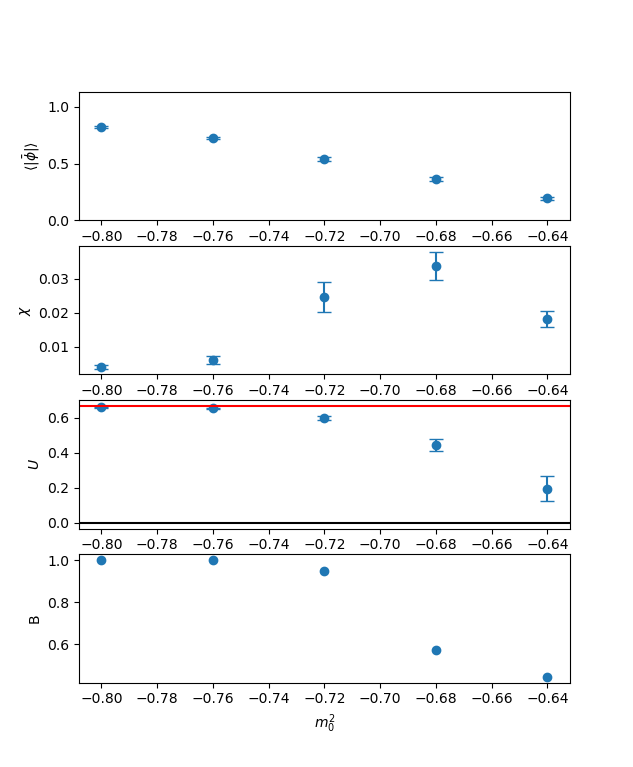
\includegraphics[width=0.7\textwidth]{imgs/phi4.png}
      \begin{subfigure}[b]{0.2\textwidth}\centering
        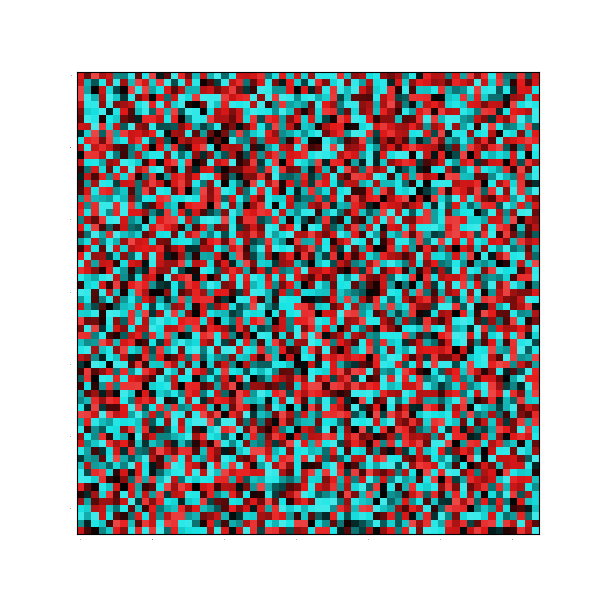
\includegraphics[width=\textwidth]{imgs/0.png}
        \caption{$\tau=0$}
      \end{subfigure}
      \hfill
      \begin{subfigure}[b]{0.2\textwidth}\centering
        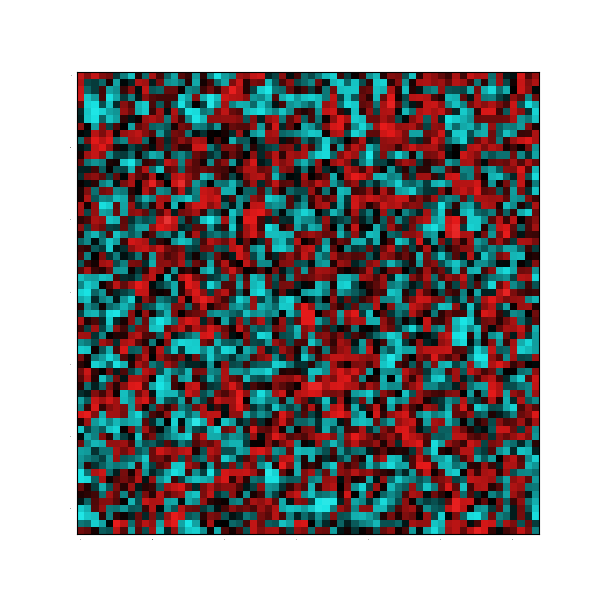
\includegraphics[width=\textwidth]{imgs/0_5.png}
        \caption{$\tau=0.5$}
      \end{subfigure}
      \hfill
      \begin{subfigure}[b]{0.2\textwidth}\centering
        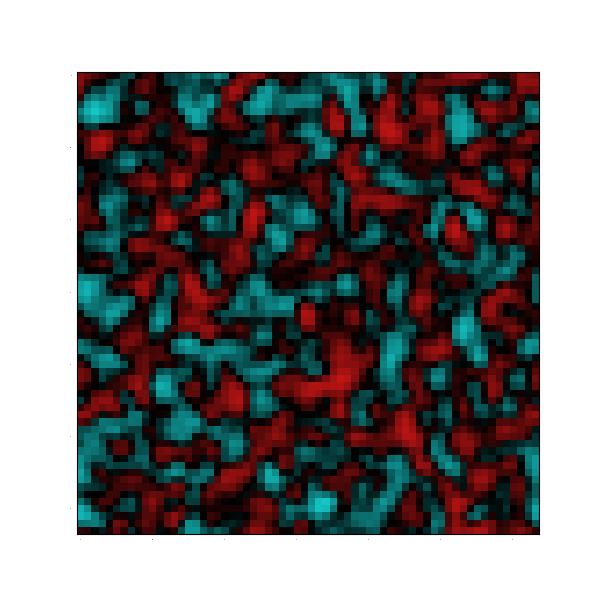
\includegraphics[width=\textwidth]{imgs/2.png}
        \caption{$\tau=2$}
      \end{subfigure}
      \hfill
      \begin{subfigure}[b]{0.2\textwidth}\centering
            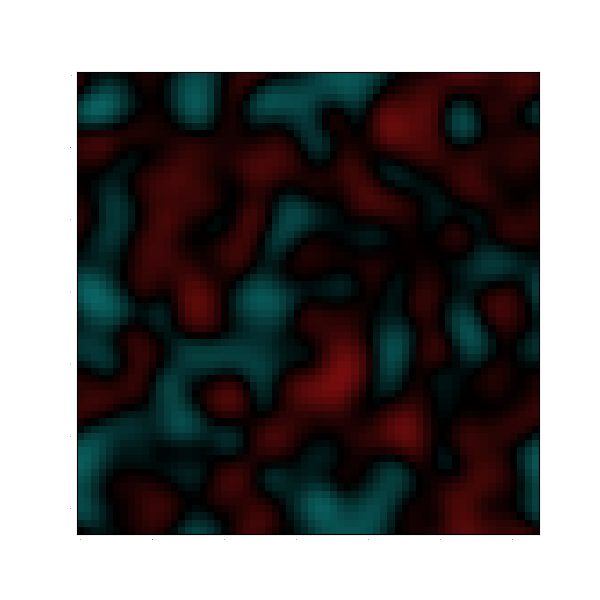
\includegraphics[width=\textwidth]{imgs/10.png}
            \caption{$\tau=10$}
      \end{subfigure}
      \hfill
      \caption{\label{fig:flow} Effect of flow time evolution on a random lattice in the symmetric phase. Red and blue indicate positive and negative values of the field in 2D spacetime.}
  
\end{figure}




\chapter{Statistical Analysis}

\chapter{Conclusion \& Outlook}


% MPI is unnecessary in this case


\appendix
\chapter{My Great Computer Program}

\section{Code sample}
\bibliographystyle{unsrt}
\bibliography{library}

\end{document}
